%% Research proposal for the study reported in papers/01-SoSym.
%% The text describes the work before the implementation and the experiments.
%% Writing rules of the project: plain words, no overclaiming, short sentences,
%% no pronouns, no em or en dashes, the long form of every abbreviation at first
%% use, and explicit connectives between sentences.
\documentclass[11pt,a4paper]{article}

\usepackage[T1]{fontenc}
\usepackage[utf8]{inputenc}
\usepackage[margin=25mm]{geometry}
\usepackage{graphicx}
\usepackage{booktabs}
\usepackage{array}
\usepackage{enumitem}
\usepackage{microtype}
\usepackage[hyphens]{url}
\usepackage[hidelinks]{hyperref}
\usepackage{titlesec}

\titleformat{\section}{\normalfont\large\bfseries}{\thesection}{0.6em}{}
\titleformat{\subsection}{\normalfont\normalsize\bfseries}{\thesubsection}{0.6em}{}
\setlist{noitemsep, topsep=4pt}
\renewcommand{\arraystretch}{1.2}

\title{\vspace{-12mm}\textbf{Towards Decentralized Model Persistence}\\[2mm]
\large Research proposal for a study of content-addressed storage in model-driven engineering}
\author{Alfa Yohannis\\
\small Department of Informatics, Pradita University\\
\small Kabupaten Tangerang, Banten, Indonesia\\
\small \href{mailto:alfa.ryano@pradita.ac.id}{alfa.ryano@pradita.ac.id}}
\date{September 2026}

\begin{document}
\maketitle

\begin{center}
\begin{tabular}{@{}ll@{}}
\toprule
Duration & 12 months \\
Target venue & Software and Systems Modeling (SoSyM), with an earlier conference paper \\
 & on the two of the research questions \\
\bottomrule
\end{tabular}
\end{center}

\section{Summary}

Model-driven engineering (MDE) stores models in files and in repositories, and a model refers to another model through an address. In the Eclipse Modeling Framework (EMF), that address is a Uniform Resource Identifier (URI) such as \texttt{file://} or \texttt{platform://}, which names a location. The content at a location can change while the address stays the same, so a reference resolves to whatever the location holds at the moment of the read. The InterPlanetary File System (IPFS) inverts that relation, because the address is a content identifier (CID) computed from the content itself. A change to a model therefore produces a new address, and an existing reference keeps pointing at the version that was referenced.

The study will build a persistence layer that stores EMF models on IPFS, will work out how references between resources survive when identifiers change on every modification, and will measure the cost. The outcome is a working artifact, an evaluation on generated models and on large reverse-engineered models, and a journal paper.

\section{Background}

EMF holds a model in a \texttt{Resource}, groups resources in a \texttt{ResourceSet}, and resolves a reference into another resource through a proxy~\cite{steinberg2008emf}. Serialization uses the XML Metadata Interchange (XMI) format, where a cross-resource reference is a URI with a fragment, for example \texttt{href="model.xmi\#//Person"}~\cite{omg2015xmi}. Research on model persistence has mainly followed scalability~\cite{kolovos2013roadmap}. Morsa stores large models in a non-relational database and loads parts on demand~\cite{pagan2015repository}. NeoEMF offers several database back ends behind one framework~\cite{daniel2017neoemf}. The Connected Data Objects (CDO) repository stores and versions models on a central server~\cite{cdo}. Hawk indexes large collections of models held in version control systems~\cite{barmpis2013hawk}.

Content addressing comes from a different tradition. Venti used a hash of the block content as the identifier of a block in archival storage~\cite{quinlan2002venti}. Git stores every object under the checksum of the object content~\cite{chacon2014progit}. Nix derives component paths from cryptographic hashes, so several versions of a component coexist~\cite{dolstra2004nix}. Software Heritage preserves source code under intrinsic identifiers~\cite{dicosmo2017heritage}. IPFS combines content addressing with a peer-to-peer network~\cite{benet2014ipfs,trautwein2022ipfs}, and the InterPlanetary Name System (IPNS) adds mutable names on top of fixed identifiers.

\section{Problem statement}

A location-based address carries no information about the version behind the address. Three settings show the consequence.

First, several models in a team often reference one metamodel or one shared library model. An edit to the shared resource changes the meaning of every referring model, and no referring model records which version was intended.

Second, reverse engineering produces models of a code base. A later analysis should run on the same snapshot as an earlier analysis, yet a file path does not name a snapshot.

Third, organizations exchange models across a boundary. A path inside one organization has no meaning inside another organization, so the parties need agreed names or a shared server.

Figure~\ref{fig:pinning} contrasts the two kinds of address. A reference that names a version would remove the ambiguity in all three settings. Content addressing offers such a reference, yet the model persistence frameworks of MDE assume a stable address with changing content. The assumption runs through the resource, the factory, the URI handler and the serialization of references, so the transfer is not a configuration change.

\begin{figure}[htbp]
\centering
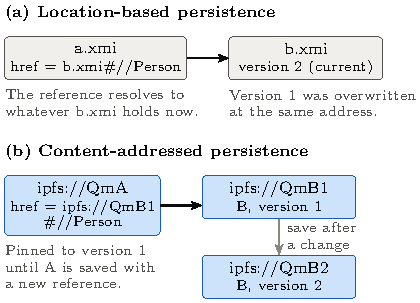
\includegraphics[width=0.62\textwidth]{../papers/01-SoSym/paper/figures/version-pinning.pdf}
\caption{Two kinds of address. (a) A file path resolves to the current content at the path. (b) A content identifier resolves to one version, so a reference keeps pointing at the version that was referenced.}\label{fig:pinning}
\end{figure}

\section{State of the art and the gap}

Three lines of work touch the problem without closing the problem.

Scalable persistence keeps identifiers stable inside a store, because the store owns the identity of an element~\cite{pagan2015repository,daniel2017neoemf,cdo}. Versioning systems such as EMFStore record operations between versions~\cite{koegel2010emfstore}, and comparison tools such as EMF Compare compute differences between two states~\cite{emfcompare}. Both lines answer the question of what changed, while neither gives an immutable address that a third party can quote.

Content-addressed storage outside MDE gives exactly such an address, and package managers already use the idea for dependencies. A lock file records an exact dependency tree, Go modules record checksums, and reproducible builds check that a binary matches the source code~\cite{npmpackagelock,lamb2022reproducible}. None of these applies content addressing to the resources and the references of a modeling framework.

The gap is therefore concrete. No reviewed approach stores EMF models under content-addressed identifiers, and no approach describes how cross-resource references behave when every save produces a new identifier.

\section{Objectives and research questions}

The study will answer three questions.

\paragraph{RQ1. Architecture.} What are the architectural challenges of extending a model persistence framework to support content-addressed decentralized storage, and how can the challenges be addressed? Sub-questions cover the mapping of \texttt{ipfs://} addresses onto the URI handling of EMF, the lifecycle of a resource that receives an identifier only after the first save, and the coexistence of file resources and content-addressed resources inside one resource set.

\paragraph{RQ2. Cross-resource references.} How can references between resources be maintained and resolved when the identifier of every resource changes on modification? Sub-questions cover the available strategies, the update of a referencing resource after a change, the treatment of reference cycles, and the publication of a model that is split into many resources.

\paragraph{RQ3. Performance.} What is the overhead of content-addressed persistence, and under which conditions is the approach practical for an MDE toolchain? Sub-questions cover the cost of a save, the cost of a load, the behaviour as the model grows, and the point where the overhead stops being acceptable for interactive work.

\begin{figure}[htbp]
\centering
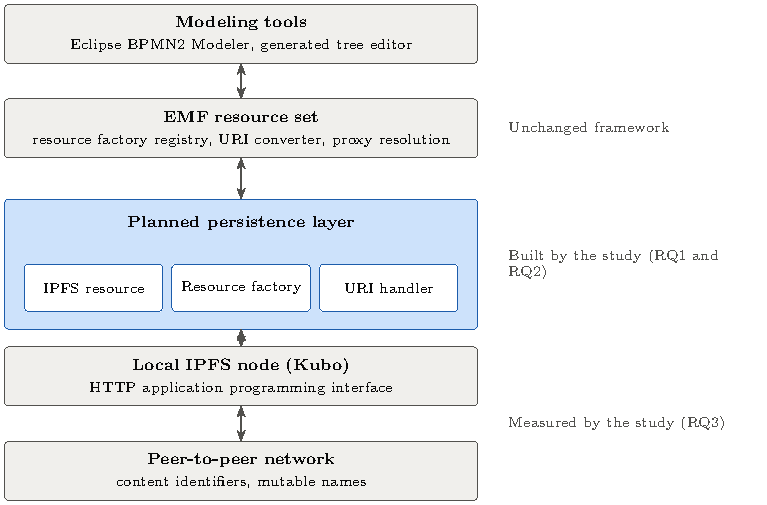
\includegraphics[width=0.82\textwidth]{figures/planned-layer.pdf}
\caption{Planned place of the persistence layer. The framework above stays unchanged, the layer in the middle is the artifact of the study, and the node below gives the storage.}\label{fig:layer}
\end{figure}

\section{Method}

The study follows design science, where a designed artifact answers the research questions and an evaluation of the artifact gives the evidence~\cite{hevner2004design}. The case study part follows the guidelines of Runeson and H\"ost~\cite{runeson2009case}. The work has four steps.

The first step analyses the problem. The analysis compares the assumptions of the EMF resource model with the properties of content addressing, and produces a list of the points where the two disagree.

The second step designs and builds the artifact. The artifact is a plugin that adds IPFS persistence to EMF, together with the strategies for references and the algorithm that updates referencing resources.

The third step validates the functions. Automated tests and example programs check save and load round trips, mixed resource sets, cross-resource references and proxy resolution.

The fourth step measures cost and scale. A benchmark on generated models compares a save through IPFS with a save to a local XMI file, and a case study on large reverse-engineered models tests the approach at a realistic size. Figure~\ref{fig:design} shows the four steps with the output of each step and with the question that each step serves.

\begin{figure}[htbp]
\centering

\includegraphics[width=\textwidth]{figures/research-design.pdf}
\caption{Research design. The four steps of the study, the output of each step, and the research question that each step serves.}\label{fig:design}
\end{figure}

\section{Work plan}

\begin{center}
\begin{tabular}{@{}p{14mm}p{112mm}p{18mm}@{}}
\toprule
Package & Work & Months \\
\midrule
WP1 & Problem analysis and literature review, with a verified reference list & 1 to 2 \\
WP2 & Persistence layer for \texttt{ipfs://} and \texttt{ipns://} (RQ1) & 2 to 5 \\
WP3 & Reference strategies, the cascade update and the publication structure (RQ2) & 4 to 8 \\
WP4 & Tool support in the Eclipse BPMN2 Modeler and in the generated tree editor & 6 to 9 \\
WP5 & Evaluation: benchmark, functional tests and the case study (RQ3) & 8 to 11 \\
WP6 & Writing, artifact release and submission & 10 to 12 \\
\bottomrule
\end{tabular}
\end{center}

Figure~\ref{fig:workplan} shows the schedule. Milestones follow the packages. M1 at month 2 is the problem analysis with the reference list. M2 at month 5 is a persistence layer that saves and loads a model through a local node. M3 at month 8 is a working update of referencing resources with tests. M4 at month 9 is the tool support inside an editor. M5 at month 11 is the complete evaluation data. M6 at month 12 is the submitted manuscript with a public artifact.

\begin{figure}[htbp]
\centering

\includegraphics[width=\textwidth]{figures/work-plan.pdf}
\caption{Schedule of the work packages over twelve months, with the six milestones.}\label{fig:workplan}
\end{figure}

\section{Evaluation plan}

The evaluation combines three methods.

Functional validation uses automated tests and example programs. The tests will cover a save and a load round trip, a resource set that holds both file resources and content-addressed resources, a reference across two resources, and the resolution of a proxy after a load in a fresh resource set.

A benchmark measures the cost. Generated models of growing size, from one hundred to several hundred thousand elements, will be saved to a local XMI file and to a local IPFS node inside the same iteration, and loaded back in a fresh resource set. Each size will run warm-up iterations followed by at least thirty measured iterations, and a paired statistical test will compare the two paths. The measurement will record the environment, because a busy machine and a node that announces new content to the network both distort the numbers.

A case study tests the approach at a realistic size. Reverse-engineered models of the Eclipse Java development tools, produced with MoDisco~\cite{bruneliere2014modisco}, give roughly one gigabyte of models across several repositories. The case study will publish the models on IPFS, both as one merged model and as a model split into one resource per compilation unit, and will then fetch the published copies back. Byte-level comparison and EMF Compare will check that a published model returns unchanged.

\section{Expected contributions and deliverables}

The study will deliver four contributions. The first is an EMF resource implementation that saves models on IPFS and loads models by content identifier or by IPNS name. The second is a description of the strategies for references between content-addressed resources, together with an algorithm that updates referencing resources after a change. The third is IPFS support inside two Eclipse tools, so the approach reaches a user interface. The fourth is an evaluation with generated models and with large reverse-engineered models.

The deliverables are public repositories with the plugin and the tool integrations, the evaluation scripts and result files, an archived dataset with a digital object identifier (DOI), and a journal manuscript for SoSyM. An earlier conference paper will cover the reference question, which carries the main new contribution.

\section{Risks and mitigation}

\begin{center}
\begin{tabular}{@{}p{50mm}p{44mm}p{55mm}@{}}
\toprule
Risk & Effect & Mitigation \\
\midrule
The resource model of EMF resists a changing identifier & The persistence layer stays incomplete & Early proof of concept in WP2, with a placeholder address before the first save \\
A reference cycle cannot settle under immutable identifiers & Some models fall outside the approach & Detect cycles before publication, and report the limit honestly \\
The update of referencing resources becomes expensive on a large graph & The approach fails at scale & Measure on the case study model, and compare a scan with an index built from manifests \\
Measurements vary with the machine and with the node & The reported numbers mislead & Fixed heap, warm-up iterations, an idle machine, a node without network announcements, and a paired test \\
A published model becomes unavailable & The evaluation cannot be repeated & Pin the content on a node under project control, and archive the dataset under a DOI \\
\bottomrule
\end{tabular}
\end{center}

\section{Resources and budget}

The core work needs one researcher, a development machine and a local IPFS node. The evaluation beyond a single machine needs rented nodes, because a claim about decentralized persistence needs more than one node. The table gives indicative categories. Amounts follow institutional rates and current provider prices, so the figures stay open until the submission of the financial form.

\begin{center}
\begin{tabular}{@{}p{40mm}p{105mm}@{}}
\toprule
Category & Purpose \\
\midrule
Personnel & Principal researcher, plus a part-time assistant for the evaluation scripts and the dataset \\
Virtual machines & Two to five nodes on different networks for the distributed measurements, for twelve months \\
Storage and pinning & Retention of the published dataset during and after the project \\
Archiving & Deposit of the dataset under a digital object identifier \\
Publication & Open access fee, if the open access route is chosen, since the subscription route carries no fee \\
Travel & One conference presentation of the reference paper \\
\bottomrule
\end{tabular}
\end{center}

\begin{thebibliography}{99}
\small

\bibitem{benet2014ipfs}
Benet, J.: IPFS, content addressed, versioned, peer-to-peer file system. arXiv:1407.3561 (2014). \url{https://arxiv.org/abs/1407.3561}

\bibitem{barmpis2013hawk}
Barmpis, K., Kolovos, D.: Hawk, towards a scalable model indexing architecture. In: BigMDE 2013, pp. 1 to 9. ACM (2013). \url{https://doi.org/10.1145/2487766.2487769}

\bibitem{bruneliere2014modisco}
Bruneli\`ere, H., Cabot, J., Dup\'e, G., Madiot, F.: MoDisco, a model driven reverse engineering framework. Information and Software Technology 56(8), 1012 to 1032 (2014). \url{https://doi.org/10.1016/j.infsof.2014.04.007}

\bibitem{cdo}
Eclipse Foundation: CDO Model Repository. \url{https://eclipse.dev/cdo/}

\bibitem{chacon2014progit}
Chacon, S., Straub, B.: Pro Git, 2nd edition. Apress, Berkeley (2014). \url{https://git-scm.com/book/en/v2}

\bibitem{daniel2017neoemf}
Daniel, G., Suny\'e, G., Benelallam, A., Tisi, M., Vernageau, Y., G\'omez, A., Cabot, J.: NeoEMF, a multi-database model persistence framework for very large models. Science of Computer Programming 149, 9 to 14 (2017). \url{https://doi.org/10.1016/j.scico.2017.08.002}

\bibitem{dicosmo2017heritage}
Di Cosmo, R., Zacchiroli, S.: Software Heritage, why and how to preserve software source code. In: iPRES 2017, pp. 1 to 10. \url{https://hal.science/hal-01590958}

\bibitem{dolstra2004nix}
Dolstra, E., de Jonge, M., Visser, E.: Nix, a safe and policy-free system for software deployment. In: LISA 2004, pp. 79 to 92. USENIX, Berkeley (2004). \url{https://www.usenix.org/legacy/publications/library/proceedings/lisa04/tech/dolstra.html}

\bibitem{emfcompare}
Eclipse Foundation: EMF Compare. \url{https://eclipse.dev/emfcompare/}

\bibitem{hevner2004design}
Hevner, A.R., March, S.T., Park, J., Ram, S.: Design science in information systems research. MIS Quarterly 28(1), 75 to 106 (2004). \url{https://doi.org/10.2307/25148625}

\bibitem{koegel2010emfstore}
Koegel, M., Helming, J.: EMFStore, a model repository for EMF models. In: ICSE 2010, vol. 2, pp. 307 to 308. ACM (2010). \url{https://doi.org/10.1145/1810295.1810364}

\bibitem{kolovos2013roadmap}
Kolovos, D.S., Rose, L.M., Matragkas, N., Paige, R.F., et al.: A research roadmap towards achieving scalability in model driven engineering. In: BigMDE 2013, pp. 1 to 10. ACM (2013). \url{https://doi.org/10.1145/2487766.2487768}

\bibitem{lamb2022reproducible}
Lamb, C., Zacchiroli, S.: Reproducible builds, increasing the integrity of software supply chains. IEEE Software 39(2), 62 to 70 (2022). \url{https://doi.org/10.1109/MS.2021.3073045}

\bibitem{npmpackagelock}
npm Docs: package-lock.json. \url{https://docs.npmjs.com/cli/v10/configuring-npm/package-lock-json}

\bibitem{omg2015xmi}
Object Management Group: XML Metadata Interchange (XMI) specification, version 2.5.1 (2015). \url{https://www.omg.org/spec/XMI/2.5.1}

\bibitem{pagan2015repository}
Espinazo Pag\'an, J., S\'anchez Cuadrado, J., Garc\'ia Molina, J.: A repository for scalable model management. Software and Systems Modeling 14(1), 219 to 239 (2015). \url{https://doi.org/10.1007/s10270-013-0326-8}

\bibitem{quinlan2002venti}
Quinlan, S., Dorward, S.: Venti, a new approach to archival storage. In: FAST 2002, pp. 89 to 101. USENIX, Berkeley (2002). \url{https://www.usenix.org/legacy/events/fast02/quinlan.html}

\bibitem{runeson2009case}
Runeson, P., H\"ost, M.: Guidelines for conducting and reporting case study research in software engineering. Empirical Software Engineering 14(2), 131 to 164 (2009). \url{https://doi.org/10.1007/s10664-008-9102-8}

\bibitem{steinberg2008emf}
Steinberg, D., Budinsky, F., Paternostro, M., Merks, E.: EMF, Eclipse Modeling Framework, 2nd edition. Addison-Wesley, Upper Saddle River (2008).

\bibitem{trautwein2022ipfs}
Trautwein, D., Raman, A., Tyson, G., Castro, I., Scott, W., Schubotz, M., Gipp, B., Psaras, Y.: Design and evaluation of IPFS, a storage layer for the decentralized web. In: ACM SIGCOMM 2022, pp. 739 to 752. ACM (2022). \url{https://doi.org/10.1145/3544216.3544232}

\end{thebibliography}

\end{document}
